%!TEX root = *.tex
%%%%%%%%%%%%%%%%%%
% カウンタのリセット
\setcounter{figure}{0}
% 問題文
{
\begin{wrapfigure}{r}{20zw}
  \vspace{-\intextsep}
  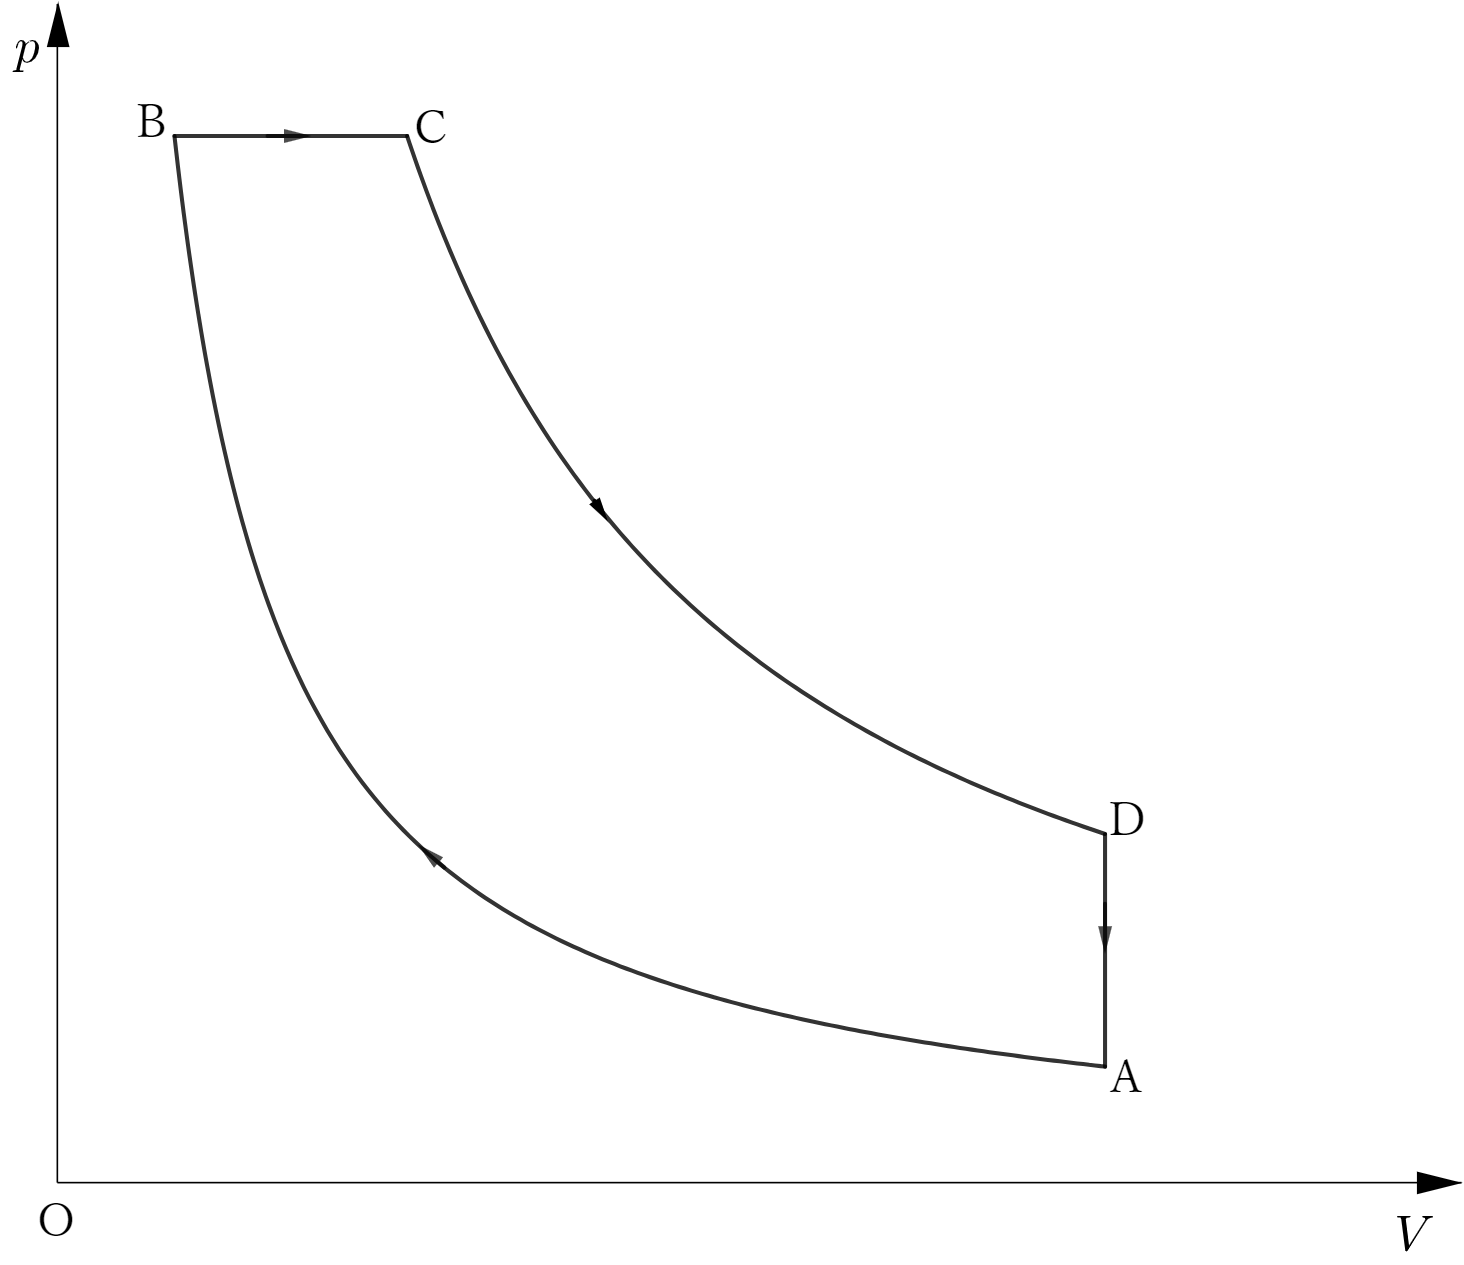
\includegraphics[width=20zw]{../graphs/jumon_69.png}
  \caption{}
\end{wrapfigure}
\nn\unit{mol}の単原子分子理想気体をピストンがついたシリンダーの中に封入して図のように体積$V$と圧力$P$を$\A\to\B\to\C\to\D\to\A$と変化させる.
$\A\to\B$と$\C\to\D$の変化はそれぞれ熱の出入りがないようにして状態の変化を行った.
さらに,$\B\to\C$の変化は圧力を一定に保って,また$\D\to\A$の変化は体積を一定に保ってそれぞれ状態の変化を行った.
状態A,B,C,Dの絶対温度をそれぞれ$T_{\A}$,$T_{\B}$,$T_{\C}$,$T_{\D}$とし,
この気体の定積モル比熱を$C_v$,定圧モル比熱を$C_p$とする.
また,ピストンとシリンダーの間に摩擦はないものとする.
次の問いに答えよ.

\par}

\begin{enumerate}[(1)]
  \setlength{\leftskip}{-1.5zw}
  \setlength{\itemindent}{1zw}\setlength{\labelsep}{0.5zw}
  \setlength{\labelwidth}{1zw}\setlength{\leftmargin}{1zw}
  \setlength{\itemsep}{0.5\baselineskip}
  \item 各過程における気体の内部エネルギーの変化$\Delta U_{\A\B},\,\Delta U_{\B\C},\,\Delta U_{\C\D},\,\Delta U_{\D\A}$を求めよ.
  \item 各過程における気体が吸収する熱量$Q_{\A\B},\,Q_{\B\C},\,Q_{\C\D},\,Q_{\D\A}$を求めよ.
  \item 各過程における気体がする仕事$W_{\A\B},\,W_{\B\C},\,W_{\C\D},\,W_{\D\A}$を求めよ.
  \item このサイクルを熱機関とみなした時の熱効率$e$を求めよ.ただし定積モル比熱と定圧モル比熱との比を$\gamma =\dfrac{C_p}{C_v}$として,$\gamma$と絶対温度を使って表せ.
\end{enumerate}






% メモ
\begin{comment}

\end{comment}


%%%%%%%%%%%%%%%%%%
